\documentclass{article}[18pt]
\usepackage{../../../format}
\lhead{MCS Coursework}
\rhead{mbkb74}
\usepackage{natded}
\lstset
{
	language=[LaTeX]TeX,
	breaklines=true,
	basicstyle=\tt\scriptsize,
}





\begin{document}
\begin{center}
\textbf{\Large Discrete Mathematics and Linear Algebra}
\end{center}
Approximately 10 hours was spent on this coursework
\begin{enumerate}
	\item \textit{Prove \textit{using induction}, that the following holds for all $n\geqslant 1$}:\hfill
[12 marks]

	$$2(\sqrt{n+1}-1)<1+\dfrac{1}{\sqrt{2}}+...+\dfrac{1}{\sqrt{n}}<2\sqrt{n}$$
	$ $\\
	\textbf{Base case:} n=1 
	$$2(\sqrt{1+1}-1)<1<2\sqrt{1}$$
	This holds\\
\\
\textbf{Proving the 1st half \cite{rosen}}\\
$$ Let \ P(n) \ be \  2(\sqrt{n+1}-1)<\dfrac{1}{\sqrt{1}}+\dfrac{1}{\sqrt{2}}+...+\dfrac{1}{\sqrt{n}}$$
\textbf{Basis step: P(1) is true}
$$2(\sqrt{2}-1)<1$$
\textbf{Inductive step: Assume that P(k) is true}
$$2(\sqrt{k+1}-1)+\dfrac{1}{\sqrt{k+1}}<\dfrac{1}{\sqrt{1}}+\dfrac{1}{\sqrt{2}}+...+\dfrac{1}{\sqrt{k}}+\dfrac{1}{\sqrt{k+1}}$$
\textbf{By showing that $2(\sqrt{k+1}-1)+\dfrac{1}{\sqrt{k+1}}>2(\sqrt{k+2}-1)$ it follows that P(k+1) is true}
$$2(\sqrt{k+2}-\sqrt{k+1})<\dfrac{1}{\sqrt{k+1}}$$
$$2(\sqrt{k+2}+\sqrt{k+1})(\sqrt{k+2}+\sqrt{k+1})<\dfrac{\sqrt{k+1}}{\sqrt{k+1}}+\dfrac{\sqrt{k+2}}{\sqrt{k+1}}$$
$$2<1+\dfrac{\sqrt{k+2}}{\sqrt{k+1}}$$
$$1<\dfrac{\sqrt{k+2}}{\sqrt{k+1}}$$
$$1<\dfrac{k+2}{k+1}$$
$$k+1<k+2$$
$$1<2$$
$$0<1$$
Trivially True, so true for P(k+1) and so by induction, since the statement is true for n=1, and that it is valid for n=k+1 if it is valid for k, we can conclude that is it valid for all positive integers \\
$$2(\sqrt{n+1}-1)<\dfrac{1}{\sqrt{1}}+\dfrac{1}{\sqrt{2}}+...+\dfrac{1}{\sqrt{n}}$$
\newpage
\textbf{Proving the second half}
$$Let \ P(n) \ be \dfrac{1}{\sqrt{1}}+\dfrac{1}{\sqrt{2}}+...+\dfrac{1}{\sqrt{n}}<2\sqrt{n}$$
\textbf{Inductive step: Assume that P(k) is true}
$$\dfrac{1}{\sqrt{1}}+\dfrac{1}{\sqrt{2}}+...+\dfrac{1}{\sqrt{k}}<2\sqrt{k}$$
\textbf{Is it true for P(k+1)}
$$\dfrac{1}{\sqrt{1}}+\dfrac{1}{\sqrt{2}}+...+\dfrac{1}{\sqrt{k}}+\dfrac{1}{\sqrt{k+1}}<2\sqrt{k}+\dfrac{1}{\sqrt{k+1}}$$
\textbf{By showing that $2\sqrt{k+1}>2\sqrt{k}+\dfrac{1}{\sqrt{k+1}}$ it follows that P(k+1) is true}	
$$2(\sqrt{k+1}-\sqrt{k})>\dfrac{1}{\sqrt{k+1}}$$
\textbf{Multiply by $\sqrt{k+1}+\sqrt{k}$}
$$2(1)>\dfrac{\sqrt{k+1}+\sqrt{k}}{\sqrt{k+1}}$$
$$2>1+\dfrac{\sqrt{k}}{\sqrt{k+1}}$$
$$1>\dfrac{\sqrt{k}}{\sqrt{k+1}}$$
$$1>\dfrac{k}{k+1}$$
$$k+1>k$$
$$1>0$$
Trivially True, so true for P(k+1) and so by induction, since the statement is true for n=1, and that it is valid for n=k+1 if it is valid for k, we can conclude that is it valid for all positive integers \\
$$\dfrac{1}{\sqrt{1}}+\dfrac{1}{\sqrt{2}}+...+\dfrac{1}{\sqrt{n}}<2\sqrt{n}$$
Since the statement is true for n=1, and that it is valid for n=k+1 if it is valid for k, we can conclude that is it valid for all positive integers \\
\\
As $2(\sqrt{n+1}-1)<\dfrac{1}{\sqrt{1}}+\dfrac{1}{\sqrt{2}}+...+\dfrac{1}{\sqrt{n}}$ is true, and $\dfrac{1}{\sqrt{1}}+\dfrac{1}{\sqrt{2}}+...+\dfrac{1}{\sqrt{n}}<2\sqrt{n}$ is true, it follows that:
	$$2(\sqrt{n+1}-1)<1+\dfrac{1}{\sqrt{2}}+...+\dfrac{1}{\sqrt{n}}<2\sqrt{n}$$







\newpage
	\item \textit{Four fair dice are thrown. What is more likely; to get exactly one 6 or to get four different numbers?} \hfill [8 marks]\\
	\\
	To get exactly one 6, there is a probability of:
	$$\dfrac{1}{6}\times(\frac{5}{6})^3$$
	per dice, so multiplying by 4 gives
	$$\dfrac{125}{324}$$
	\\
	On the first dice, there is a probability of 1 there is a new number, on the second dice, there is a probability of $\frac{5}{6}$ there is a new number, on the 3rd $\frac{4}{6}$ and on the fourth $\frac{3}{6}$
	$$1\times\frac{5}{6}\times \frac{4}{6}\times\frac{3}{6}=\frac{5}{18}$$
	$\dfrac{5}{18}<\dfrac{125}{324}$ so it is more likely to get one 6.
	
	
	
	
	
	\newpage
	\item\textit{ Letters A, B, C, and D are listed in random order. Let X be the random variable
	equal to the number of pairs of letters not in alphabetical order (for example, in
	CADB, such pairs are CA, CB, and DB). Find the expected value and the variance
	of X} \hfill[10 marks]\\
	\begin{tabular}{|c|c|}
		\hline 
		Ordering & Pairs not in order (X) \\ 
		\hline 
		ABCD & 0 \\ 
		\hline 
		ABDC & 1 \\ 
		\hline 
		ACBD & 1 \\ 
		\hline 
		ACDB & 2 \\ 
		\hline 
		ADBC & 2 \\ 
		\hline 
		ADCB & 3 \\ 
		\hline 
		BACD & 1 \\ 
		\hline 
		BADC & 2 \\ 
		\hline 
		BCAD & 2 \\ 
		\hline 
		BCDA & 3 \\ 
		\hline 
		BDAC & 3 \\ 
		\hline 
		BDCA & 4 \\ 
		\hline 
		CABD & 2 \\ 
		\hline 
		CADB & 3 \\ 
		\hline 
		CBAD & 3 \\ 
		\hline 
		CBDA & 4 \\ 
		\hline 
		CDAB & 4 \\ 
		\hline 
		CDBA & 5 \\ 
		\hline 
		DABC & 3 \\ 
		\hline 
		DACB & 4 \\ 
		\hline 
		DBAC & 4 \\ 
		\hline 
		DBCA & 5 \\ 
		\hline 
		DCAB & 5 \\ 
		\hline 
		DCBA & 6 \\ 
		\hline 
	\end{tabular} 
$$p(x=0)=\dfrac{1}{24}$$
$$p(x=1)=\dfrac{3}{24}$$
$$p(x=2)=\dfrac{5}{24}$$
$$p(x=3)=\dfrac{6}{24}$$
$$p(x=4)=\dfrac{5}{24}$$
$$p(x=5)=\dfrac{3}{24}$$
$$p(x=6)=\dfrac{1}{24}$$
$$E(X)=0\times\dfrac{1}{24}+
1\times\dfrac{3}{24}+
2\times\dfrac{5}{24}+
3\times\dfrac{6}{24}+
4\times\dfrac{5}{24}+
5\times\dfrac{3}{24}+
6\times\dfrac{1}{24}=3$$
$$E(X^2)=0^2\times\dfrac{1}{24}+
1^2\times\dfrac{3}{24}+
2^2\times\dfrac{5}{24}+
3^2\times\dfrac{6}{24}+
4^2\times\dfrac{5}{24}+
5^2\times\dfrac{3}{24}+
6^2\times\dfrac{1}{24}=\dfrac{67}{6}$$
$$Var(X)=E(X^2)-E(X)^2=\dfrac{67}{6}-3^2=\dfrac{13}{6}$$
\newpage
	
	
	
	\item \textit{For each integer $q\geqslant 2$ determine whether the complete bipartite graph $K_{3,q}$ is KO-reducible, and if so find its KO number} \hfill [20 marks]
	\begin{figure}[H]
		\begin{center}
			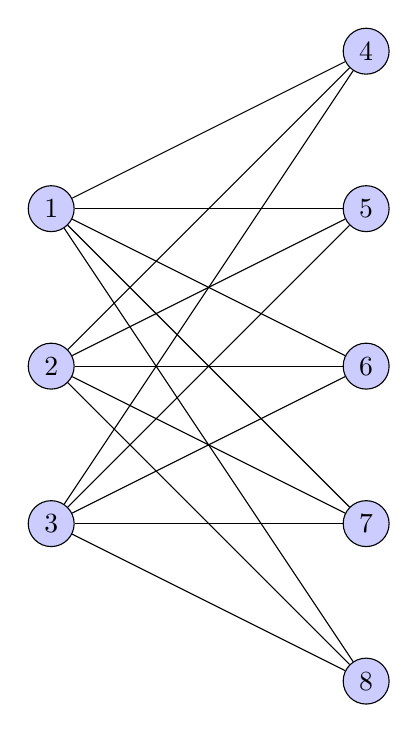
\begin{tikzpicture}[main_node/.style={circle,fill=blue!20,draw,minimum size=1em,inner sep=3pt]}]
			
			\node[main_node] (3) at (0,2) {3};
			\node[main_node] (2) at (0,4) {2};
			\node[main_node] (1) at (0,6) {1};
			\node[main_node] (8) at (4,0) {8};
			\node[main_node] (7) at (4,2) {7};
			\node[main_node] (6) at (4,4) {6};
			\node[main_node] (5) at (4,6) {5};
			\node[main_node] (4) at (4,8) {4};
			
			\draw (1) -- (4);
			\draw (2) -- (4);
			\draw (3) -- (4);
			\draw (1) -- (5);
			\draw (2) -- (5);
			\draw (3) -- (5);
			\draw (1) -- (6);
			\draw (2) -- (6);
			\draw (3) -- (6);
			\draw (1) -- (7);
			\draw (2) -- (7);
			\draw (3) -- (7);
			\draw (1) -- (8);
			\draw (2) -- (8);
			\draw (3) -- (8);
			\end{tikzpicture}
		\end{center}
		\caption{$K_{3,5}$}
		\label{K3,5}
	\end{figure}
Consider the complete bipartite graph to be made of two sets, set A on the left hand side has 3 elements. Set B on the right hand side has q elements.\\
\\
As in each round each element from each set must select an element from the other set, at a minimum one element from each set will be removed per round.\\
 This means that there is a maximum of 3 rounds as after that set A will be empty, as it contains 3 elements. In this case where the minimum number of elements is removed from set A each turn, there will be 3, then 2, then 1, then 0 elements in that set. This means that the maximum that could be removed from set B in this case is 3 elements, then 2 elements, then 1 element, if all the elements of set A were to choose different elements from set B. This means that if $q>6$ then set B could not be emptied before set A. Therefore for any $q>6$ the graph will not be KO-Reducible.\\
\\
This means that when the number of knockouts that can be performed on set B are:
\begin{itemize}
	\item 3 in round 1
	\item 2 in round 2 - meaning up to 5 can be knocked out at the end of round 2
	\item 1 in round 3 - meaning up to 6 can be knocked out at the end of round 3
\end{itemize}
This means that:
\begin{itemize}
\item $q=3$ has a KO number of 1
\item $q=4$ and $q=5$ have a KO number of 2
\item $q=6$ has a KO number of 3
\end{itemize}	
However importantly this does not mean that $q=2$ can be knocked out in one round, as in this case set 2 is the smaller set, so in one round, all of set 2 could be knocked out, but there would be an element remaining in set 1. So in cases where $|Set \ A|>|Set \ B|$, instead of trying to remove the maximal number from set B and the minimal from set A, it should be the other way round.\\
Because of the remaining condition that one needs to be knocked out from each set per round, by removing one from set B each round, 2 can be removed from set A in the first round and 1 in the second, resulting in a KO number of 2 for $q=2$ \\
\\
$q=4$ is treated slightly differently as it is not on one of the maximums for a round. This means that if the elements from set B were to be deleted maximally it would not be KO reducible. Instead, in the first round, two of the elements from set A need to select one element from set B, allowing the second round to have 2 elements in each set, which select each other to reduce to nothing.\\
\\
Method:
Consider the two sets A ($S_A$) and B ($S_B$), below is outlined how many from each set should be selected per round:\\
\\
\textbf{q=2: KO 2}
\begin{itemize}
	\item 1st round $S_A$:2, $S_B$:1
	\item 2nd round $S_A$:1, $S_B$:1
\end{itemize}
\textbf{q=3: KO 1}
\begin{itemize}
	\item 1st round $S_A$:3, $S_B$:3
\end{itemize}
\textbf{q=4: KO 2}
\begin{itemize}
	\item 1st round $S_A$:1, $S_B$:2
	\item 2nd round $S_A$:2, $S_B$:2
\end{itemize}
\textbf{q=5: KO 2}
\begin{itemize}
	\item 1st round $S_A$:1, $S_B$: 3
	\item 2nd round $S_A$:2, $S_B$:2
\end{itemize}
\textbf{q=6: KO 3}
\begin{itemize}
	\item 1st round $S_A$:1, $S_B$:3
	\item 2nd round $S_A$:1, $S_B$:2
	\item 3rd round $S_A$:1, $S_B$:1
\end{itemize}
\newpage
\section{Graphs}
Below is shown the nodes to be selected from the graph in each turn in order for it to be KO reducible. When all the nodes are selected, no nodes will exist in the next round, so it has been reduced.
\subsection{q=2}
	\begin{figure}[H]
	\begin{center}
		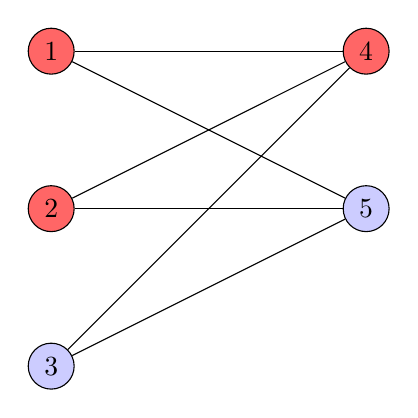
\begin{tikzpicture}[main_node/.style={circle,fill=blue!20,draw,minimum size=1em,inner sep=3pt]},select_node/.style={circle,fill=red!60,draw,minimum size=1em,inner sep=3pt]}]
		
		\node[main_node] (3) at (0,2) {3};
		\node[select_node] (2) at (0,4) {2};
		\node[select_node] (1) at (0,6) {1};
		\node[main_node] (6) at (4,4) {5};
		\node[select_node] (5) at (4,6) {4};
		
		
		\draw (1) -- (5);
		\draw (2) -- (5);
		\draw (3) -- (5);
		\draw (1) -- (6);
		\draw (2) -- (6);
		\draw (3) -- (6);
		\end{tikzpicture}
	\end{center}
	\caption{$K_{3,2}$ - Round 1}
	\label{K3,5}
\end{figure}
	\begin{figure}[H]
	\begin{center}
		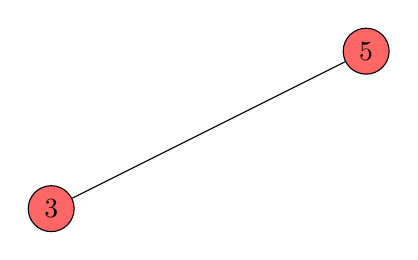
\begin{tikzpicture}[main_node/.style={circle,fill=blue!20,draw,minimum size=1em,inner sep=3pt]},select_node/.style={circle,fill=red!60,draw,minimum size=1em,inner sep=3pt]}]
		
		\node[select_node] (3) at (0,2) {3};
		\node[select_node] (6) at (4,4) {5};
		
		\draw (3) -- (6);
		\end{tikzpicture}
	\end{center}
	\caption{$K_{3,2}$ - Round 2}
	\label{K3,5}
\end{figure}		
\subsection{q=3}	
	\begin{figure}[H]
	\begin{center}
		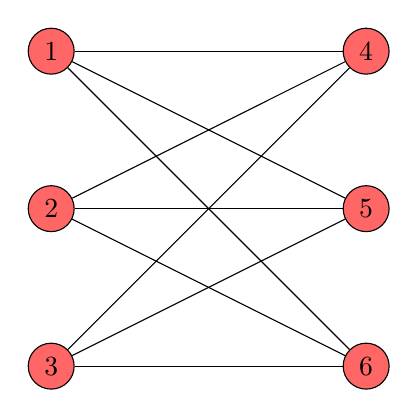
\begin{tikzpicture}[main_node/.style={circle,fill=blue!20,draw,minimum size=1em,inner sep=3pt]},select_node/.style={circle,fill=red!60,draw,minimum size=1em,inner sep=3pt]}]
		
		\node[select_node] (3) at (0,2) {3};
		\node[select_node] (2) at (0,4) {2};
		\node[select_node] (1) at (0,6) {1};
		\node[select_node] (7) at (4,2) {6};
		\node[select_node] (6) at (4,4) {5};
		\node[select_node] (5) at (4,6) {4};
		
		
		\draw (1) -- (5);
		\draw (2) -- (5);
		\draw (3) -- (5);
		\draw (1) -- (6);
		\draw (2) -- (6);
		\draw (3) -- (6);
		\draw (1) -- (7);
		\draw (2) -- (7);
		\draw (3) -- (7);
		\end{tikzpicture}
	\end{center}
	\caption{$K_{3,3}$ - Round 1}
	\label{K3,3}
\end{figure}
\subsection{q=4}
	\begin{figure}[H]
	\begin{center}
		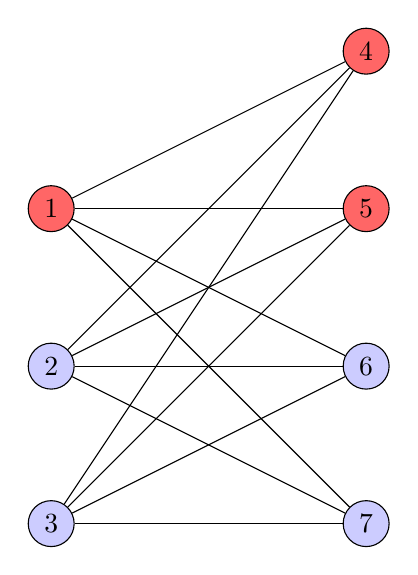
\begin{tikzpicture}[main_node/.style={circle,fill=blue!20,draw,minimum size=1em,inner sep=3pt]},select_node/.style={circle,fill=red!60,draw,minimum size=1em,inner sep=3pt]}]
		
		\node[main_node] (3) at (0,2) {3};
		\node[main_node] (2) at (0,4) {2};
		\node[select_node] (1) at (0,6) {1};
		\node[main_node] (7) at (4,2) {7};
		\node[main_node] (6) at (4,4) {6};
		\node[select_node] (5) at (4,6) {5};
		\node[select_node] (4) at (4,8) {4};
		
		\draw (1) -- (4);
		\draw (2) -- (4);
		\draw (3) -- (4);
		\draw (1) -- (5);
		\draw (2) -- (5);
		\draw (3) -- (5);
		\draw (1) -- (6);
		\draw (2) -- (6);
		\draw (3) -- (6);
		\draw (1) -- (7);
		\draw (2) -- (7);
		\draw (3) -- (7);
		\end{tikzpicture}
	\end{center}
	\caption{$K_{3,4}$ - Round 1}
	\label{K3,4}
\end{figure}
	\begin{figure}[H]
	\begin{center}
		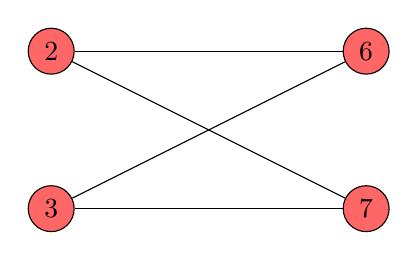
\begin{tikzpicture}[main_node/.style={circle,fill=blue!20,draw,minimum size=1em,inner sep=3pt]},select_node/.style={circle,fill=red!60,draw,minimum size=1em,inner sep=3pt]}]
		
		\node[select_node] (3) at (0,2) {3};
		\node[select_node] (2) at (0,4) {2};
		\node[select_node] (7) at (4,2) {7};
		\node[select_node] (6) at (4,4) {6};
		

		\draw (2) -- (6);
		\draw (3) -- (6);
		\draw (2) -- (7);
		\draw (3) -- (7);
		\end{tikzpicture}
	\end{center}
	\caption{$K_{3,4}$ - Round 2}
	\label{K3,4}
\end{figure}
\subsection{q=5}

	\begin{figure}[H]
	\begin{center}
		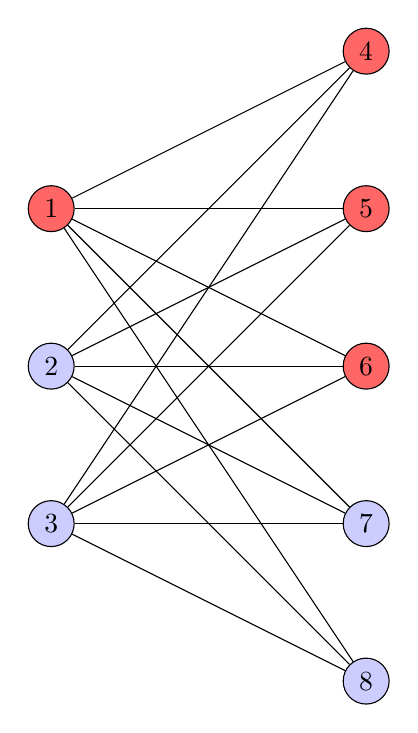
\begin{tikzpicture}[main_node/.style={circle,fill=blue!20,draw,minimum size=1em,inner sep=3pt]},select_node/.style={circle,fill=red!60,draw,minimum size=1em,inner sep=3pt]}]
		
		\node[main_node] (3) at (0,2) {3};
		\node[main_node] (2) at (0,4) {2};
		\node[select_node] (1) at (0,6) {1};
		\node[main_node] (8) at (4,0) {8};
		\node[main_node] (7) at (4,2) {7};
		\node[select_node] (6) at (4,4) {6};
		\node[select_node] (5) at (4,6) {5};
		\node[select_node] (4) at (4,8) {4};
		
		\draw (1) -- (4);
		\draw (2) -- (4);
		\draw (3) -- (4);
		\draw (1) -- (5);
		\draw (2) -- (5);
		\draw (3) -- (5);
		\draw (1) -- (6);
		\draw (2) -- (6);
		\draw (3) -- (6);
		\draw (1) -- (7);
		\draw (2) -- (7);
		\draw (3) -- (7);
		\draw (1) -- (8);
		\draw (2) -- (8);
		\draw (3) -- (8);
		\end{tikzpicture}
	\end{center}
	\caption{$K_{3,5}$ - Round 1}
	\label{K3,5}
\end{figure}
	\begin{figure}[H]
	\begin{center}
		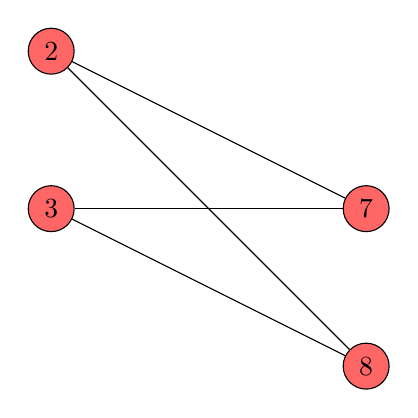
\begin{tikzpicture}[main_node/.style={circle,fill=blue!20,draw,minimum size=1em,inner sep=3pt]},select_node/.style={circle,fill=red!60,draw,minimum size=1em,inner sep=3pt]}]
		
		\node[select_node] (3) at (0,2) {3};
		\node[select_node] (2) at (0,4) {2};
		
		\node[select_node] (8) at (4,0) {8};
		\node[select_node] (7) at (4,2) {7};
		
		
		
		\draw (2) -- (7);
		\draw (3) -- (7);
		
		\draw (2) -- (8);
		\draw (3) -- (8);
		\end{tikzpicture}
	\end{center}
	\caption{$K_{3,5}$ - Round 2}
	\label{K3,5}
\end{figure}
\subsection{q=6}
	\begin{figure}[H]
	\begin{center}
		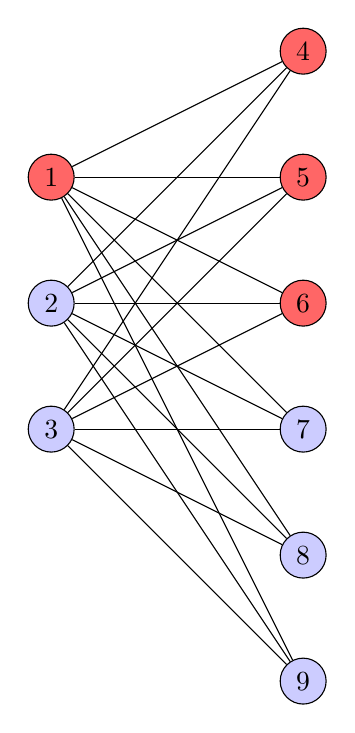
\begin{tikzpicture}[main_node/.style={circle,fill=blue!20,draw,minimum size=1em,inner sep=3pt]},select_node/.style={circle,fill=red!60,draw,minimum size=1em,inner sep=3pt]},scale=0.8]
		
		\node[main_node] (3) at (0,2) {3};
		\node[main_node] (2) at (0,4) {2};
		\node[select_node] (1) at (0,6) {1};
		\node[main_node] (9) at (4,-2) {9};
		\node[main_node] (8) at (4,0) {8};
		\node[main_node] (7) at (4,2) {7};
		\node[select_node] (6) at (4,4) {6};
		\node[select_node] (5) at (4,6) {5};
		\node[select_node] (4) at (4,8) {4};
		
		\draw (1) -- (4);
		\draw (2) -- (4);
		\draw (3) -- (4);
		\draw (1) -- (5);
		\draw (2) -- (5);
		\draw (3) -- (5);
		\draw (1) -- (6);
		\draw (2) -- (6);
		\draw (3) -- (6);
		\draw (1) -- (7);
		\draw (2) -- (7);
		\draw (3) -- (7);
		\draw (1) -- (8);
		\draw (2) -- (8);
		\draw (3) -- (8);
		\draw (1) -- (9);
		\draw (2) -- (9);
		\draw (3) -- (9);
		\end{tikzpicture}
	\end{center}
	\caption{$K_{3,6}$ - Round 1}
	\label{K3,6}
\end{figure}
	\begin{figure}[H]
	\begin{center}
		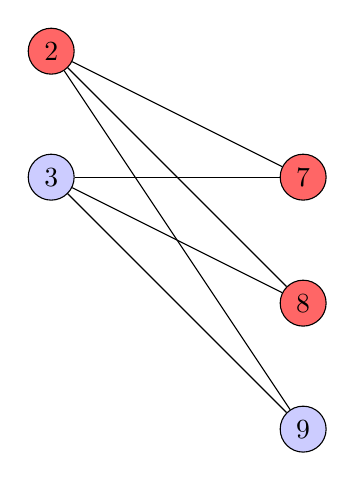
\begin{tikzpicture}[main_node/.style={circle,fill=blue!20,draw,minimum size=1em,inner sep=3pt]},select_node/.style={circle,fill=red!60,draw,minimum size=1em,inner sep=3pt]},scale=0.8]
		
		\node[main_node] (3) at (0,2) {3};
		\node[select_node] (2) at (0,4) {2};
		\node[main_node] (9) at (4,-2) {9};
		\node[select_node] (8) at (4,0) {8};
		\node[select_node] (7) at (4,2) {7};

		


		\draw (2) -- (7);
		\draw (3) -- (7);

		\draw (2) -- (8);
		\draw (3) -- (8);

		\draw (2) -- (9);
		\draw (3) -- (9);
		\end{tikzpicture}
	\end{center}
	\caption{$K_{3,6}$ - Round 2}
	\label{K3,6}
\end{figure}
	\begin{figure}[H]
	\begin{center}
		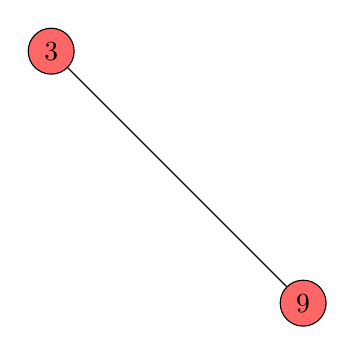
\begin{tikzpicture}[main_node/.style={circle,fill=blue!20,draw,minimum size=1em,inner sep=3pt]},select_node/.style={circle,fill=red!60,draw,minimum size=1em,inner sep=3pt]},scale=0.8]
		
		\node[select_node] (3) at (0,2) {3};
		\node[select_node] (9) at (4,-2) {9};		

		\draw (3) -- (9);
		\end{tikzpicture}
	\end{center}
	\caption{$K_{3,6}$ - Round 3}
	\label{K3,6}
\end{figure}

\newpage	
\begin{center}
	\textbf{\Large Logic and Discrete Structures}
\end{center}
	\item \textit{Let $\varphi$ be the formula $((a\land b)\Rightarrow c)\land (a\lor b)$}
	\begin{enumerate}
		\item \textit{Reduce $\varphi$ to disjunctive normal form using truth tables} \hfill [10 marks]
		\item\textit{ Reduce $\lnot \varphi$ to conjunctive normal form (without using truth tables)}\hfill [5 marks]
	\end{enumerate}
(a).\\
\begin{center}

{\renewcommand{\arraystretch}{1.2} 
\begin{tabular}{|c|c|c|c|c|c|c|cc}
	\cline{1-7}
	a & b & c & $((a\land b)$ & $\Rightarrow c)$ & $\land$ & $(a\lor b)$&&$\varphi$ \\ 
	\cline{1-7}
	F & F & F & F & T & \textbf{F} & F&&F \\  
	\cline{1-7}
	F & F & T & F & T & \textbf{F} & F&&F \\ 
	\cline{1-7} 
	F & T & F & F & T & \textbf{T} & T&&T \\ 
	\cline{1-7} 
	F & T & T & F & T & \textbf{T} & T&&T \\ 
	\cline{1-7}
	T & F & F & F & T & \textbf{T} & T&&T \\ 
	\cline{1-7} 
	T & F & T & F & T & \textbf{T} & T&&T \\ 
	\cline{1-7}
	T & T & F & T & F & \textbf{F} & T&&F \\ 
	\cline{1-7}
	T & T & T & T & T & \textbf{T} & T&&T \\ 
	\cline{1-7}
\end{tabular}}
\end{center}
So $\varphi$ in disjunctive normal form is equivalent to:
$$(\lnot a \land b \land \lnot c)\lor (\lnot a \land b \land c)\lor (a \land \lnot b \land \lnot c)\lor (a \land \lnot b \land c)\lor (a \land b \land c)$$
So the cnf of $\lnot \psi$ is 
$$(a \lor \lnot b \lor c)\land ( a \lor \lnot b \lor \lnot c)\land (\lnot a \lor  b \lor  c)\land (\lnot a \lor b \lor \lnot c)\land (\lnot a \lor \lnot b \lor \lnot c)$$


\item \textit{Is the set $\{\land,\oplus\}$, where $p\oplus q \equiv \lnot(p\Leftrightarrow q)$, functionally complete?} \hfill [5 marks]\\

Suppose that $\{\land,\oplus \}$ is functionally complete. If it is functionally complete, then there is a formula using only $\{\land,\oplus\}$ such that
$$\varphi\equiv\lnot p$$
$p\land p$ is false if p is false\\
$p\oplus p$ is false if p is false\\
\\
Hence $\varphi$ cannot exist, so the set is not functionally complete

\item \textit{Prove the following sequents using natural deduction. In your proofs you may (only) use the rules $\land i, \land e1, \land e2, \lnot \lnot i, \lnot\lnot e\\, \Rightarrow e, \Rightarrow i, \lor i1, \lor i2, \lor e, \bot e, \lnot e, \lnot i$ and the Law of the Excluded Middle. At each step mention the rule you have applied. You may write $\lor i$ for $\lor i1$ and $\lor i2$. Similarly, you may write $\land e$ for $\land e1$ and $\land e2$}
\begin{enumerate}
\item $\lnot a\land b\land (a\lor(b\Rightarrow c))\vdash c\lor d$ \hfill [10 marks]



\item $a\lor(\lnot b\land \lnot c\land \lnot d)\vdash (a\lor b)\land (a\lor \lnot c)\land (a\lor \lnot d)$ \hfill [10 marks]
\end{enumerate}
(a)
\[
\Jproof{
	\proofline{\lnot a \land b \land (a\lor (b\Rightarrow c))}{Premise}
	\proofline{\lnot a}{$\land$ e (1)}
	\proofline{\lnot b}{$\land$ e (1)}
	\proofline{\lnot a\lor(b\Rightarrow c)}{$\land$ e (1)}
	\cablk{
		\proofline{a}{Assumption}
		\proofline{\bot}{$\lnot$ e (2) (5)}
		\proofline{b\Rightarrow c}{$\bot$ e (6)}
	}	
	\cablk{
		\proofline{b\Rightarrow c}{Assumption}
		\proofline{b\Rightarrow c}{copy (8)}
	}
	\proofline{b\Rightarrow c}{$\lor$ e (4) (5-7)(8-9)}
	\proofline{c}{$\Rightarrow$ e (3) (10)}
	\proofline{c\lor d}{$\lor$ i (11)}
}		
\]
(b)
\[
\Jproof{
	\proofline{a\lor (\lnot b\land \lnot c\land \lnot d)}{Premise}
	\cablk{
		\proofline{a}{Assumption}
		\proofline{a\lor \lnot b}{$\lor$ i (2)}
	}	
	\cablk{
		\proofline{\lnot b\land \lnot c\land \lnot d}{Assumption}
		\proofline{\lnot b}{$\land$ e (4)}
		\proofline{a\lor \lnot b}{$\lor$ i (5)}
	}	
	\proofline{a\lor \lnot b}{$\lor$ e (1) (2-3) (4-6)}
	\cablk{
		\proofline{a}{Assumption}
		\proofline{a\lor \lnot c}{$\lor$ i (8)}
	}
	\cablk{
		\proofline{\lnot b\land \lnot c\land \lnot d}{Assumption}
		\proofline{\lnot c}{$\land$ e (10)}
		\proofline{a\lor \lnot c}{$\lor$ i (11)}
	}
	\proofline{a\lor \lnot c}{$\lor$ e (1) (8-9) (10-12)}
	\cablk{
		\proofline{a}{Assumption}
		\proofline{a\lor \lnot d}{$\lor$ i (14)}
	}
	\cablk{
		\proofline{\lnot b\land \lnot c\land \lnot d}{Assumption}
		\proofline{\lnot d}{$\land$ e (16)}
		\proofline{a\lor \lnot d}{$\lor$ i (17)}
	}
	\proofline{a\lor \lnot d}{$\lor$ e (1) (14-15) (16-18)}
	\proofline{(a\lor\lnot b)\land (a\lor \lnot c)}{$\land$ i (7)(13)}
	\proofline{(a\lor\lnot b)\land(a\lor \lnot c)\land (a\lor \lnot d)}{$\land$ i (19) (20)}
}		
\]


\newpage
\item L\textit{et $\varphi$ be the formula $\neg ( a \land ( \neg a \lor \neg b ) \land ( b \lor c ) \land ( \neg c \lor \neg d \lor e ) \land ( e \lor d ) \land ( \neg e \lor \neg c ) )$. Is $\varphi$ a theorem? Use resolution to answer this question. Mention on which clauses you use resolution each time you apply it} \hfill [10 marks]
$$Let \ \varphi = \neg ( a \land ( \neg a \lor \neg b ) \land ( b \lor c ) \land ( \neg c \lor \neg d \lor e ) \land ( e \lor d ) \land ( \neg e \lor \neg c ) )$$
$$Therefore \ \lnot \varphi =  a \land ( \neg a \lor \neg b ) \land ( b \lor c ) \land ( \neg c \lor \neg d \lor e ) \land ( e \lor d ) \land ( \neg e \lor \neg c ) $$
So the set of clauses to which we apply resolution is:
$$a \qquad \lnot a \lor \lnot b \qquad b\lor c \qquad \lnot c\lor \lnot d \lor e \qquad e\lor d \qquad \lnot e\lor\lnot c$$
\begin{enumerate}[label=(\arabic*)]
	\item a
	\item $\lnot a \lor \lnot b$
	\item $b\lor c$
	\item $\lnot c \lor \lnot d \lor e$
	\item $e\lor d$
	\item $\lnot e\lor \lnot c$
	\item $\lnot b \qquad$ \hfill(1,2)
	\item $c\qquad$ \hfill (3,7)
	\item $\lnot d\lor e\qquad$ \hfill (4,8)
	\item $e\lor e$ \hfill (5,9)
	\item $e\qquad$ \hfill (10)  
	\item $\lnot c$ \hfill (6,11)
	\item $\varnothing$ \hfill (8,12) 
\end{enumerate}
This results in the empty set, so $\varphi$ is a theorem

\end{enumerate}
\newpage
\bibliographystyle{unsrt}
\bibliography{bibliography}
\end{document}